\documentclass[12pt]{article}
\usepackage[utf8]{inputenc}
\usepackage[T2A]{fontenc}
\usepackage[russian]{babel}
\usepackage{graphicx}
\usepackage{wrapfig}
\usepackage{amsmath}
\usepackage{amssymb}
\usepackage{array}
\usepackage{geometry}
\usepackage{fancyhdr}
\usepackage{booktabs}
\usepackage{caption}
\usepackage{float}
\usepackage{indentfirst}
\usepackage{setspace}
\usepackage{titlesec}
\usepackage{physics}

% Настройка полей
\geometry{a4paper, left=2.5cm, right=2.5cm, top=2.5cm, bottom=2.5cm}

% Настройка стиля разделов
\titleformat{\section}[block]{\Large\bfseries\centering}{\thesection}{1em}{}
\titleformat{\subsection}[block]{\large\bfseries}{\thesubsection}{1em}{}

% Настройка межстрочного интервала
\onehalfspacing

% Настройка колонтитулов
\pagestyle{fancy}
\fancyhf{}
\fancyhead[R]{\thepage}
\fancyhead[L]{Работа 3.4.5: Петля гистерезиса (динамический метод)}
\renewcommand{\headrulewidth}{0.4pt}

% Уменьшение отступа перед и после формул
\setlength{\abovedisplayskip}{8pt}
\setlength{\belowdisplayskip}{8pt}
\setlength{\abovedisplayshortskip}{8pt}
\setlength{\belowdisplayshortskip}{8pt}

% Отключение нумерации формул
\renewcommand{\theequation}{}
\usepackage{amsmath}
\makeatletter
\renewcommand{\theequation}{}
\makeatother

\begin{document}

\begin{center}
  \LARGE\textbf{Работа 3.4.5}\\[0.3cm]
  \LARGE\textbf{Петля гистерезиса (динамический метод)}\\[0.4cm]
  \large\textit{Чекмарев Игорь}\\[0.2cm]
  \rule{\textwidth}{0.4pt}
\end{center}

\vspace{0.5cm}

\noindent\textbf{Цель работы:} изучение петель гистерезиса различных ферромагнитных материалов в переменных полях.

\vspace{0.3cm}

\noindent\textbf{В работе используются:} автотрансформатор, понижающий трансформатор, интегрирующая цепочка, амперметр, вольтметр, электронный осциллограф (ЭО), делитель напряжения, тороидальные образцы с двумя обмотками.

\section*{Теория}
Гистерезис - явление, при котором состояние системы зависит не только от значения внешних параметров в данный момент, но и от предыдущего состояния системы.

Магнитную индукцию удобно определять с помощью ЭДС, возникающей при изменении потока в катушке, намотанной на образец. Пусть катушка плотно обхватывает образец, а индукция $\vec{B}$ однородна. Тогда
$$
\varepsilon \mathscr{E} = -\dfrac{d\Phi}{dt}, \Phi = BSN_\text{и} \Rightarrow |B|=\dfrac{1}{SN_\text{и}}\int \mathscr{E}dt,
$$
где $N_\text{и}$ -- число витков в измерительной катушке, $S$ -- площадь витка. То есть для определения $B$ нужно проинтегрировать сигнал, наведённый на измерительную катушку.\\
Используя интегрирующую схему из конденсатора $C$ опротивления $R \gg \dfrac{1}{\Omega C}$ ($\Omega$ -- частота сигнала в сети), с учётом $U_{\text{вых}} \ll U_{\text{вх}}$, получим
$$
U_{\text{вых}}=\dfrac{1}{C}\int Idt \approx \dfrac{1}{RC}\int U_{\text{вх}}dt
$$
Если $R_{\text{и}}$ и $C_{\text{и}}$ -- параметры интегрирующей ячейки, то получим
$$
|B| = \dfrac{R_{\text{и}}C_{\text{и}}}{SN_\text{и}}U_{\text{вых}}
$$
\section*{Описание работы} 
\begin{center}
\includegraphics[scale=0.5]{схема гистерезис.png}
\end{center}
Схема установки представлена на рисунке. Напряжение сети с помощью регулировочного трансформатора Ат через разделительный понижающий трансформатор Тр подаётся на намагничивающую обмотку $N_0$ образца. Значение тока в обмотке измеряется амперметром А, с ним последовательно сопротивление $R_0$, напряжение с которого подается на вход Х электронного осциллографа (ЭО). Это напряжение пропорционально току в обмотке $N_0$, а значит и напряжённости магнитного поля $H$ в образце.\\
Для измерения магнитной индукции $B$ в обмотке $N_\text{и}$ на вход интегрирующей цепочки подаётся напряжение $U_\text{и}$, пропорциональное $\dfrac{dB}{dt}$, а с выхода снимается напряжение $U_C$, пропорциональное $B$, которое подаётся на вход Y ЭО.\\
Кривая, возникающая на экране, воспроизводит петлю гистерезиса. По формулам 
$$
H = \dfrac{IN_0}{2\pi R}, B = \dfrac{R_\text{и} C_\text{и}U_\text{вых}}{SN_\text{и}}
$$
где $I = K_X/R_0, U_\text{вых} = K_Y$, $K_X, K_Y$ -- чувствительность усилителя ЭФ соответствующих шкал, можно провести калиброку ЭО.\\
При закороченной обмотке $N_0$ амперметр измеряет эффективное значение синусоидального тока $I_\text{эф}$ через сопротивление $R_0$. Если $2x$ -- длина горизонтальной прямой на экране, то чувствительность канала Х
$$
m_X = \dfrac{2\sqrt{2}R_0I_\text{эф}}{2x}
$$
При отключённом тороиде сигнал с обмотки 12.6 В подаётся на делитель, и его часть снимается с делителя с каоэффициетном деления и подаётся на Y ЭО вместо $U_C$. Вольтметр измеряет напряжение $U_\text{эф}$ на этих клеммах делителя. Если $2y$ -- длина вертикальной прямой на экране, то чувствительность канал Y
$$
m_Y = \dfrac{2\sqrt{2}U_\text{эф}}{2y}
$$
Если измерить с помощью ЭО поочерёдно амлитуды сигналов $U_\text{вх}$ и $U_\text{вых}$ $RC$-цепочки, можно рассчитать постоянную времени 
$$
\tau = RC = \dfrac{U_\text{вх}}{\Omega U_\text{вых}} 
$$

\section*{Ход работы и обработка результатов}
\begin{enumerate}
\item Собираем схему, подключаем в сеть. Параметры установки $R_\text{и} = 20~\text{кОм}, C_\text{и} = 20~\text{мкФ}, R_0 = 0.2~\text{Ом}$. Параметры образцов:
\begin{table}[h]
\centering
\begin{tabular}{|c|c||c||c|}
\hline
      & Феррит 1000нм & Пермаллой & Кремнистое железо \\ \hline
$N_0$    & 42            & 20        & 25                \\ \hline
$N_\text{и}$    & 400           & 300       & 250               \\ \hline
$S$, м$^2$     & 3        & 0.76  & 2            \\ \hline
$2\pi R$, cv & 25          & 13.3     & 11              \\ \hline
\end{tabular}
\end{table}
\item Подбираем ток питания и коэффициенты усиления ЭО так, чтобы предельная петля гистерезиса занимала большую часть экрана. Зарисуем предельную петлю на кальке.
\item Снимаем на ту же кальку начальную кривую намагничивания: плавно уменьшая ток намагничивания до нуля, будем отмечать на кальке вершины наблюдаемых частных петель. Кривая, соединяющая эти вершины, проходит вблизи начальной кривой намагничивания. 
\item Восстановим предельную петлю. Измерим на экране двойные амплитуды для коэрцитивной силы и индукции насыщения. Соответствующие значения $K_X$ и $K_Y$.\\
Вычислим цену деления ЭО для петли в А/м по оси Х и в теслах на деление для оси Y.
\item Отключим намагничивающую обмотку от цепи, соединив оба провода, идущих к обмотке, на одной из её клемм. Рассчитаем чувствительность канала X.
\item Разберём цепь тороида. Соединим вход Y ЭО с клеммами делителя "1/100-земля" и подключим вольтметр к тем же точкам делителя. Рассчитаем чувствительность канала X.
\begin{table}[t]
\centering
\begin{tabular}{|c|c|c||c|c||c|c|}
\hline
\multirow{}{}{} & \multicolumn{2}{c||}{Феррит 1000нм} & \multicolumn{2}{c||}{Пермаллой} & \multicolumn{2}{c|}{Кремнистое железо} \\ \cline{2-7} 
                  & Значение          & $\sigma$          & Значение        & $\sigma$        & Значение            & $\sigma$            \\ \hline
$K_X$, В/дел              & 0.050             & 0.002          & 0.050           & 0.002        & 0.200               & 0.002            \\ \hline
$K_Y$, В/дел              & 0.020             & 0.001          & 0.050           & 0.002        & 0.050               & 0.001            \\ \hline
$I$, А               & 0.483             & 0.009          & 0.223           & 0.005        & 2.18               & 0.03            \\ \hline
$H$, А/м*дел             & 42             & 1.5           & 37.6           & 1.5         & 227                 & 5                \\ \hline
$B$, Тл/дел              & 0.067             & 0.003          & 0.88            & 0.04         & 0.40                & 0.03            \\ \hline
$x$, см                 & 3.60              & 0.05           & 2.00            & 0.05         & 3.80                & 0.05             \\ \hline
$y$, см                 & 3.20              & 0.05           & 1.80            & 0.05         & 2.60                & 0.05             \\ \hline
$[x]$, см              & 0.55              & 0.05              & 0.80              & 0.05              & 0.40              & 0.05              \\ \hline
$[y]$, см              & 1.40              & 0.05              & 1.70              & 0.05              & 0.95              & 0.05              \\ \hline \hline
$I_{\text{эф}}$, А             & 0.60             & 0.005          & 0.65           & 0.005        & 2.32               & 0.005            \\ \hline
$m_X$                & 0.040            & 0.001         & 0.041          & 0.001       & 0.183              & 0.001           \\ \hline
\hline
$U_{\text{эф}}$, В               & 0.0395            & 0.0001         & 0.124          & 0.001       & 0.124              & 0.001           \\ \hline
$m_Y$                 & 0.0175            & 0.0003         & 0.0464          & 0.0008       & 0.0464              & 0.0008           \\ \hline
\end{tabular}
\end{table}
\item Для определения напряжений на входе и выходе интегрирующей соединим вход ячейки с обмоткой "6,3 В" трансформатора. 
Подключим Y-вход ЭО ко входу интегрирующей ячейки и отключим Х-вход ЭО. Определим входное напряжение на RC-цепочке: $U_{\text{вх}} = 14.2 \pm 0.2~\text{В}$.
Не меняя тока, переключим Y-вход ЭО к выходу ячейки  и аналогичным образом определим напряжение $U_{\text{вых}}= 0.108 \pm 0.002~\text{В}$. Тогда (с учётом $\nu = \frac{\omega}{2\pi} = 50~\text{Гц}$)
\begin{center}
\fbox{$\tau = \dfrac{U_\text{вх}}{\Omega U_\text{вых}} = \frac{14.2}{100\pi *0.108} =  0.42 \pm 0.09~\text{с}$}
\end{center}
Рассчитывая через параметры цепи, $\tau = R_\text{и} C_\text{и} = 0.4~\text{c}$, что близко к полученному.

\item  Рассчитаем коэрцитивную силу и индукцию насыщения для каждого образца и сравним с табличными:
\begin{center}
\fbox{$\mu_ = \dfrac{1}{\mu_0}\frac{dB}{dH}$}

\begin{table}[h]
\centering
\begin{tabular}{|c|c|c||c|c||c|c|}
\hline
\multirow{}{}{} & \multicolumn{2}{c||}{Феррит 1000нм} & \multicolumn{2}{c||}{Пермаллой} & \multicolumn{2}{c|}{Кремнистое железо} \\ \cline{2-7} 
                  & Значение         & $\sigma$           & Значение       & $\sigma$          & Значение           & $\sigma$              \\ \hline
$H_c$, А/м           & 23.1         & 1        & 30     & 1.6      & 90           & 4          \\ \hline
Таблица           & \multicolumn{2}{c||}{16 - 1600}           & \multicolumn{2}{c||}{4}  & \multicolumn{2}{c|}{40}              \\ \hline
$B_s$, Тл            & 0.215              & 0.01        & 1.58 & 0.2      & 1.04               & 0.1         \\ \hline
Таблица           & \multicolumn{2}{c||}{0.1 - 0.4}           & \multicolumn{2}{c||}{1.05}  & \multicolumn{2}{c|}{1.95}              \\ \hline
$\mu_{start}$           & 1590           & 40           & 18621           & 795           & 1400           & 40           \\ \hline
Таблица           & \multicolumn{2}{c||}{10 - 2000}           & \multicolumn{2}{c||}{4000}           & \multicolumn{2}{c||}{500}           \\ \hline
$\mu_{max}$           & 1900           & 80           & 42300           & 1600           & 2800           & 80           \\ \hline
Таблица           & \multicolumn{2}{c||}{ - }           & \multicolumn{2}{c||}{10000}           & \multicolumn{2}{c||}{7000}           \\ \hline
\end{tabular}
\end{table}

\begin{figure}[ht]
\centering
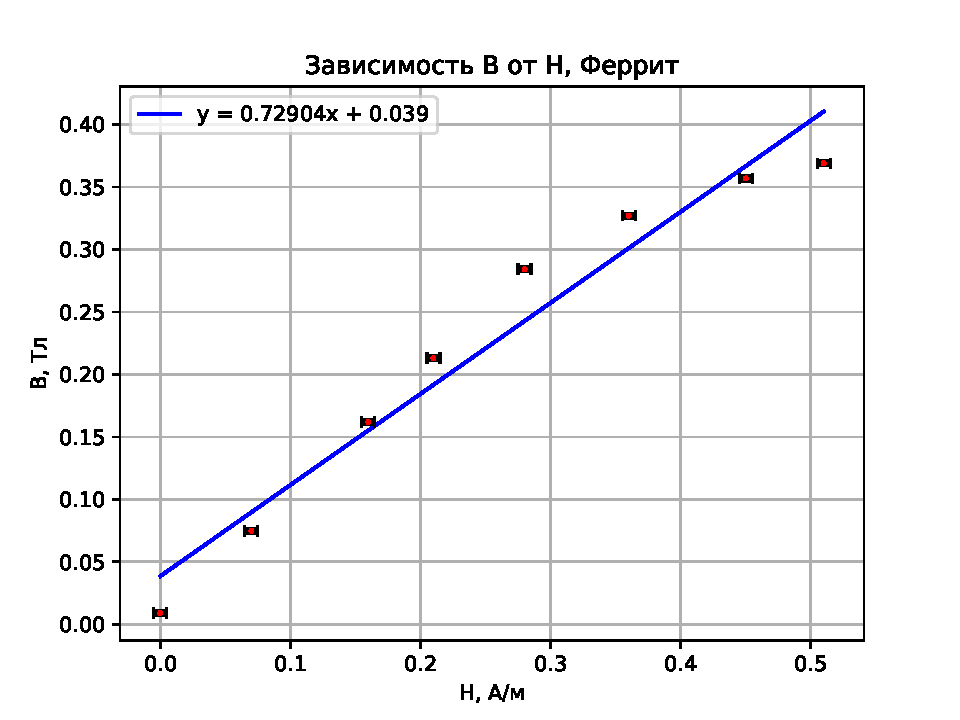
\includegraphics[width=1\textwidth]{Зависимость В от Н, Феррит.pdf}
\hfill
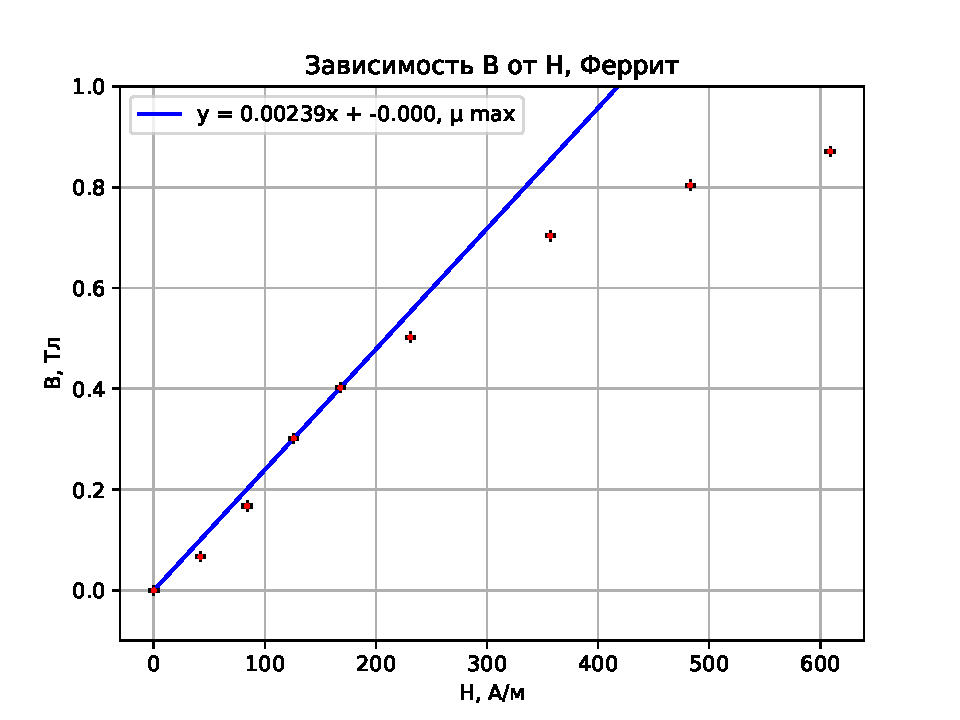
\includegraphics[width=1\textwidth]{Зависимость В от Н, Феррит, μ max.pdf}
\caption{Кривые намагничивания для феррита}
\end{figure}

\begin{figure}[ht]
\centering
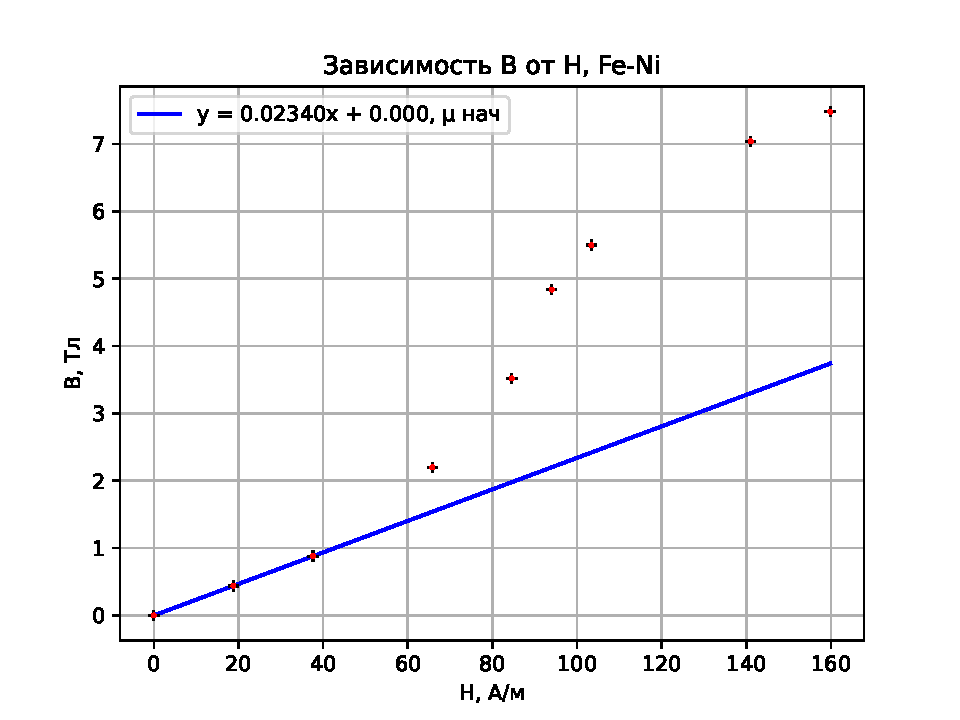
\includegraphics[width=1\textwidth]{Зависимость В от Н, Fe-Ni.pdf}
\hfill
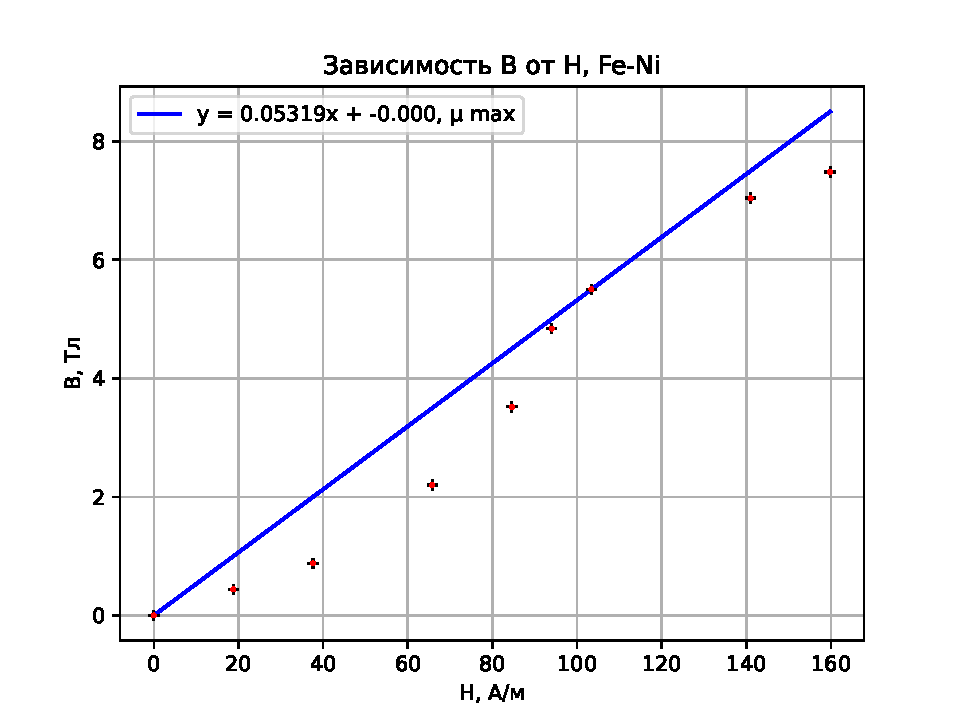
\includegraphics[width=1\textwidth]{Зависимость В от Н, Fe-Ni, μ max.pdf}
\caption{Кривые намагничивания для Fe-Ni}
\end{figure}

\begin{figure}[ht]
\centering
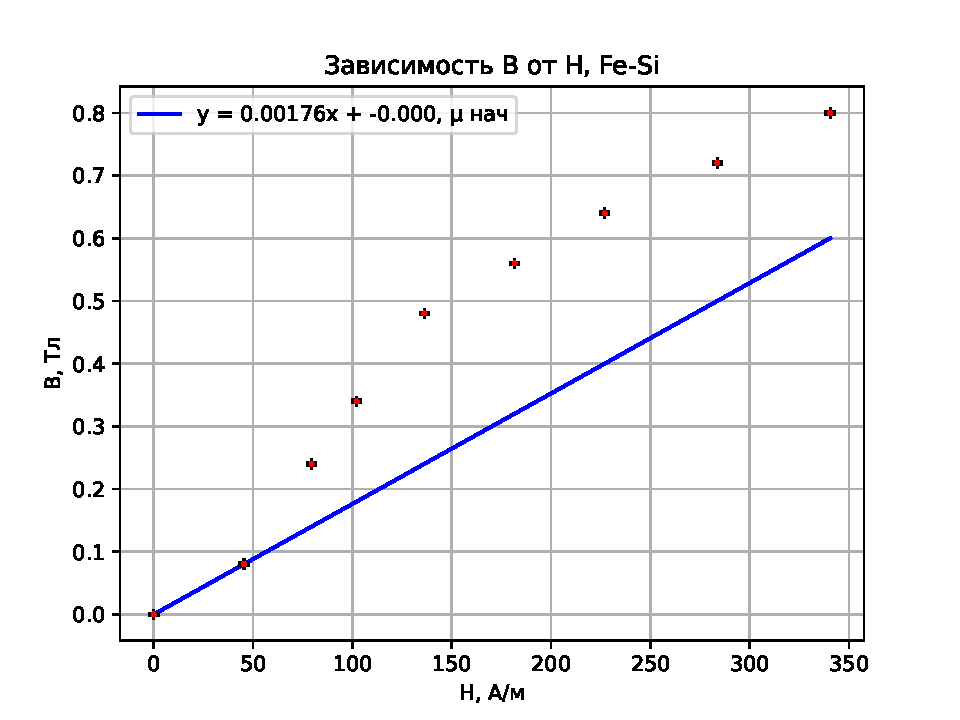
\includegraphics[width=1\textwidth]{Зависимость В от Н, Fe-Si.pdf}
\hfill
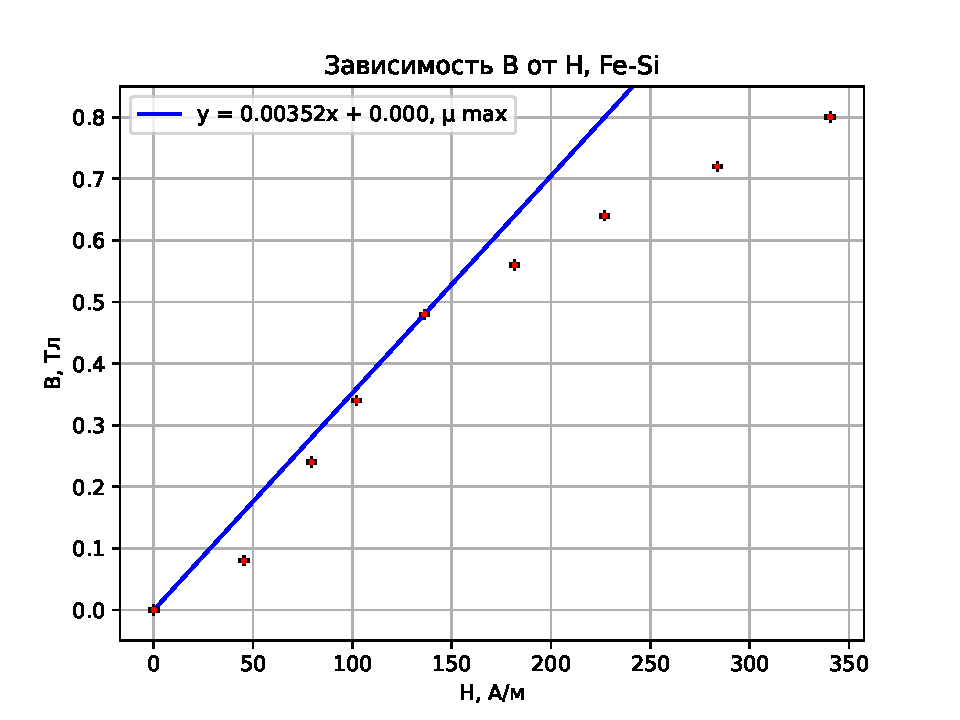
\includegraphics[width=1\textwidth]{Зависимость В от Н, Fe-Si, μ max.pdf}
\caption{Кривые намагничивания для Fe-Si}
\end{figure}

\end{enumerate}
\newpage
\newpage
\section*{Выводы}

Изучены петли гистерезиса в переменных полях для следующих материалов: феррит, пермаллой и железо кремнистое (найдены их $H_c$, $B_s$, $\mu_\text{нач}$ и $\mu_\text{max}$).
Полученные значения для феррита оказались в пределах табличных значений. Значения для кремнистого железа близки к табличным, а вот значения $H_c$ и $\mu$ для пермаллоя больше всего отличаются от табличных.

Найдена чувствительность каналов осциллографа для $H$ (A/м*дел) и $B$ (Тл/дел).

Проведена калибровка осциллографа по каналу $K_x$ для каждого из образцов, и по каналу $K_y$ для каждой из чувствительностей по этой оси (при помощи потенциометра R2 и делителя $\frac{1}{100}$. 

Найдена постоянная времени $\tau$ RC-цепочки (0.42 с). Проверено выполнение условия $R >>\frac{1}{\omega C}$: $R$ примерно в 200 раз больше $\frac{1}{\omega C}$.

\end{document}